\chapter{Hausdorff Stability Theorem} \label{chap:hausdorff-stability}

Persistence diagrams help summarize the information given by the homology groups of a filtration over a certain data set. They represent the birth and death of every feature in an easy to analice format scattering points over the upper half of the plane $\R^2 $ and its diagonal $ \Delta $. Once we have computed the diagrams given by two datasets we can measure distances between them using the bottleneck distance, enabling us to decide wether two diagrams are close to each other. However, this would be kind of useless if the bottleneck distance were not stable. If minor differences in original data would cause great changes in the bottleneck distance between the corresponding persistence diagrams, then this data summary method would be as good as any other random method.

Fortunately for us, David Cohen-Steiner, Herbert Edelsbrunner and John Harer, proved in their 2005 paper that the bottleneck distance over persistence diagrams is indeed stable \cite{Edelsbrunner}. This means that, when comparing the bottleneck distance between the persistence diagrams formed by the pre images of two tame functions, see Definition \ref{def:tame-function}, the first will be always lower or equal that the Lebesgue $L_\infty$ norm between the two functions.

Along this chapter we will follow Edelsbrunner et al. paper \cite{Edelsbrunner} to prove Theorem \ref{theorem:edelsbrunner-stability}. Recall from Definition \ref{def:critical-value} that homological critical values are the real numbers at where homology changes. Recall too the notation given in Definition \ref{def:persistent-homology}. For a triangulable topological space $X$, let $ f \colon X \to \R $ and fix some $ k \in \Z $, we denoted
\begin{equation}
    F_x \coloneq H_k(f^{-1}(-\infty, x]),
\end{equation}
and for every $ x \leq y $, we denoted the induced inclusion map from $ X_x $ to $ X_y $ as
\begin{equation}
    f_x^y \colon F_x \to F_y.
\end{equation}
The persistent homology module associated to $ x $ and $ y $ was the subspace of $X_y$ given by 
\begin{equation}
    F_x^y \coloneq \im f_x^y.
\end{equation}
The persistent Betti numbers were defined as
\begin{equation}
    \beta_x^y \coloneq \dim(F_x^y).
\end{equation}

We can define the multiplicity of each critical point as follows.

\begin{definition}[Multiplicity]
    Let $f \colon X \to \R $ be tame, and $ (a_i)_{i = 1, \dots, n} $ be its homological critical values. Take $ (b_i)_{i = 1, \dots, n} $ be an interleaved sequence of non critical values such that $ b_{i-1} < a_i < b_i $ for all $ i = 1, \dots, n $. Define $ b_{-1} = a_0 = -\infty $, $b_{n+1} = a_{n+1} = \infty $. The {\bf multiplicity} of $ (a_i, a_j) \in D(f) $, denoted $ \mu_i^j $ is
    \begin{align}
        \mu_i^j \coloneq \beta_{b_{i-1}}^{b_j} - \beta_{b_{i}}^{b_j} + \beta_{b_{i}}^{b_{j-1}} - \beta_{b_{i-1}}^{b_{j-1}}.
    \end{align}
    The {\bf total multiplicity} of a multiset A, denoted $ \#(A) $ is the sum of the multiplicities of every element in $A$.
\end{definition}

Note that the total multiplicity of a multiset is the the generalized concept of cardinality of a normal set. While the cardinality of a set counts the number of elements in the set, the multiplicity of a multiset counts how many elements, different or not, are there in the multiset.

When a function $ f $ is tame, we can form a finite multiset of barcodes taking each pair of critical points $ (a_i, a_j) $ with their corresponding multiplicity $ \mu_i^j $, for each $ 0 \leq i < j \leq n+ 1 $. Hence we can form a persistence diagram $ D(f) $. The main theorem of this chapter states that the distance of two of those persistence diagrams is never grater that the $L^\infty $ norm between the functions that form them.

\begin{restatable}[Main Theorem, \cite{Edelsbrunner}]{theorem}{Main} \label{theorem:edelsbrunner-stability}
    Let $ X $ be a triangulable space, and $ f, g\colon X \to \R $ continuous tame functions. Then,
    \begin{align}
        \db (D(f), D(g)) \leq \|f-g\|_\infty
    \end{align}
\end{restatable}

\section{Hausdorff Stability}

Before approaching the proof of Theorem \ref{theorem:edelsbrunner-stability}, this section shows how the claim of the theorem is true when the bottleneck distance is replaced by the Hausdorff distance. On Section \ref{sec:bot-stability} this assertion is used to give an upper limit of the bottleneck distance by Hausdorff distance, proving the main theorem.

We will denote the closed upper left quadrant of a point $ (x, y) \in \R^2 $ as 
\begin{equation}
    Q_x^y \coloneq [-\infty, x] \times [y, \infty].
\end{equation}

\begin{lemma}[$k$-Triangle Lemma, \cite{Edelsbrunner}] \label{lemma:k-triangle}
    Let $ f\colon X \to \R $ be a tame function, $ x < y \in \R $ be non critical values of $ f $. Then the multiplicity $\mu $ of the persistence diagram of $ f $ in the closed upper left quadrant is 
    \begin{align}
        \mu = \# (D(f) \cap Q_x^y) = \beta_x^y.
    \end{align}
\end{lemma}
\begin{proof}
    Let $ x = b_i $, $ y = b_{j-1} $.
    \begin{align} 
        \mu &= \sum_{k \leq i \leq j \leq l} \mu_k^l = \sum_{k \leq i \leq j \leq l} \beta_{b_{k-1}}^{b_l} - \beta_{b_k}^{b_l} + \beta_{b_k}^{b_{l-1}} - \beta_{b_{k-1}}^{b_{l-1}} \label{eq:k-triangle-1} \\
        &= \beta_{b_{-1}}^{b_{n+1}} - \beta_{b_i}^{b_{n+1}} + \beta_{b_i}^{b_{j-1}} - \beta_{b_{j-1}}^{b_{-1}} = \beta_{b_k}^{b_{l-1}} = \beta_x^y. \label{eq:k-triangle-2}
    \end{align}
    The fist two equalities in \eqref{eq:k-triangle-1} are just the definition of total multiplicity. In \eqref{eq:k-triangle-2}, note that every other term in the sum cancels. Then note that $ \beta_{b_{-1}}^{b_{n+1}} = \dim F_{-\infty}^{\infty} $, $ \beta_{b_i}^{b_{n+1}} = \dim F_{x}^{\infty} $ and $ \beta_{b_{j-1}}^{b_{-1}} = \dim F_{-\infty}^y $. All of them are the dimension of the trivial module, therefore, equal to $ 0 $. This leaves only one remaining term and completes the proof.
\end{proof}

Denote the {\bf upper left quadrants} $ Q \coloneq Q_b^c = [-\infty, b] \times [c, \infty] $, $ Q_\e \coloneq Q_{b-\e}^{c+\e} = [-\infty, b-\e] \times [c+\e, \infty] $.

\begin{lemma}[Quadrant Lemma, \cite{Edelsbrunner}] \label{lemma:quadrant-lemma}
    Let $f,g \colon X \to \R $ be two tame functions. With the notation abobe, the following inequality holds,
    \begin{align}
        \#(D(f), \cap Q_\e) \leq \#(D(g) \cap Q).
    \end{align}
\end{lemma}
\begin{proof}
    Let $ \e \coloneq \|f - g\|_\infty $. Hence, considering the pre-image of the functions, we have the following inclusions
    \begin{align}
        f^{-1}((-\infty, x]) &\subseteq g^{-1}((-\infty, x+\e)), \label{eq:quadrant-1}\\
        g^{-1}((-\infty, x]) &\subseteq f^{-1}((-\infty, x+\e)). \label{eq:quadrant-2}
    \end{align}
    Name $ \varphi_x \colon F_x \to G_{x+\e} $  to the inclusion map induced by \eqref{eq:quadrant-1} and $ \psi_x \colon G_x \to F_{x+\e} $ to the inclusion map induced by \eqref{eq:quadrant-2}. Let $ b<c \in \R $. With the described maps, we can form commutative diagram \eqref{cd:quadrant-1} where we observe that
    \begin{align} 
        \im(f_{c-\e}^{c+\e}) = F_{c-\e}^{c+\e} \subseteq \psi_c \circ g_b^c(G_b) = \psi_c (G_b^c).
    \end{align}
    \begin{equation} \label{cd:quadrant-1}
    \begin{tikzcd}
        F_{b-\e} \arrow[r, "f_{b-\e}^{c+\e}"] \arrow[d, "\varphi_{b-\e}"']
        & F_{c+\e} \\
        G_b \arrow[r, "g_b^c"]
        & G_c \arrow[u, "\psi_c"']        
    \end{tikzcd}
    \end{equation}
    Last inclusion is enough for the requirements of this proof, nevertheless, we will make one more note that will be useful later on, through the proof of Lemma \ref{lemma:box-lemma}. Fit the maps so that they describe commutative diagram \eqref{cd:quadrant-2}, showing that
    \begin{align}
        \psi_c(G_b^c) = \psi_c \circ g_b^c(G_b) = f_{b+\e}^{c+\e} \circ \psi_b(G_b) \subseteq F_{b+\e}^{c+\e}.
    \end{align}
    \begin{equation} \label{cd:quadrant-2}
    \begin{tikzcd}
        F_{b+\e} \arrow[r, "f_{b+\e}^{c+\e}"]
        & F_{c+\e} \\
        G_b \arrow[r, "g_b^c"] \arrow[u, "\varphi_{b}"]
        & G_c \arrow[u, "\psi_c"']        
    \end{tikzcd}
    \end{equation}
    From both diagrams we finally obtain the inclusion chain
    \begin{align}  \label{eq:quadrant-3}
        F_{c-\e}^{c+\e} \subseteq \psi_c (G_b^c) \subseteq F_{b+\e}^{c+\e}.
    \end{align}
    By Lemma \ref{lemma:k-triangle}, we are able to count the elements in the intersection of the diagrams with the upper left quadrants. Hence
    \begin{align}
        \#(D(f) \cap Q_\e) &= \beta_{b-\e}^{c+\e} = \dim F_{b-\e}^{c+\e}, \\
        \#(D(g) \cap Q) &= \beta_b^c = \dim G_b^c.
    \end{align}
    As if one homology module is contain into an other, the dimension of the first must be lower or equal to the one of the second. Also, the dimension is invariant under inclusion maps. Thus, the first inclusion of \eqref{eq:quadrant-3} asserts that $ F_{c-\e}^{c+\e} \subseteq \psi_c (G_b^c) $ and therefore we have proven that $ \dim F_{c-\e}^{c+\e} \leq  \dim G_b^c $.
\end{proof} 

We will introduce some useful notation. Let $ f\colon X \to \R $ be a tame function. Let $ w < x < y < z \in \R $ be numbers different from critical values of $ f $. Recall that $ F_x = H_k(f^{-1}(-\infty, x]) $, $ f_x^y \colon F_x \to F_y $ and $ F_x^y = \dim f_x^y $. We denote
\begin{align}
    f_x^{y, z} &\coloneq f_y^z \rvert_{F_x^y},
    \quad &
    F_x^{y, z} &\coloneq \dim f_x^{y, z}.
\end{align}
Note, from linear algebra, that $ \dim F_x^{y,z} = \dim F_x^y - \dim F_x^z $. Also note that $ F_w^y \subseteq F_x^y $. Therefore, $ \ker F_w^y \subseteq \ker F_x^y $ and we can define the quotient
\begin{align}
    F_{w,x}^{y,z} \coloneq F_x^{y,z} / F_w^{y,z}.
\end{align}
Figure \ref{fig:homology-modules} (from \cite{Edelsbrunner}) depicts a visual interpretation and recap of this notation

\begin{figure}[h]
    \centering
    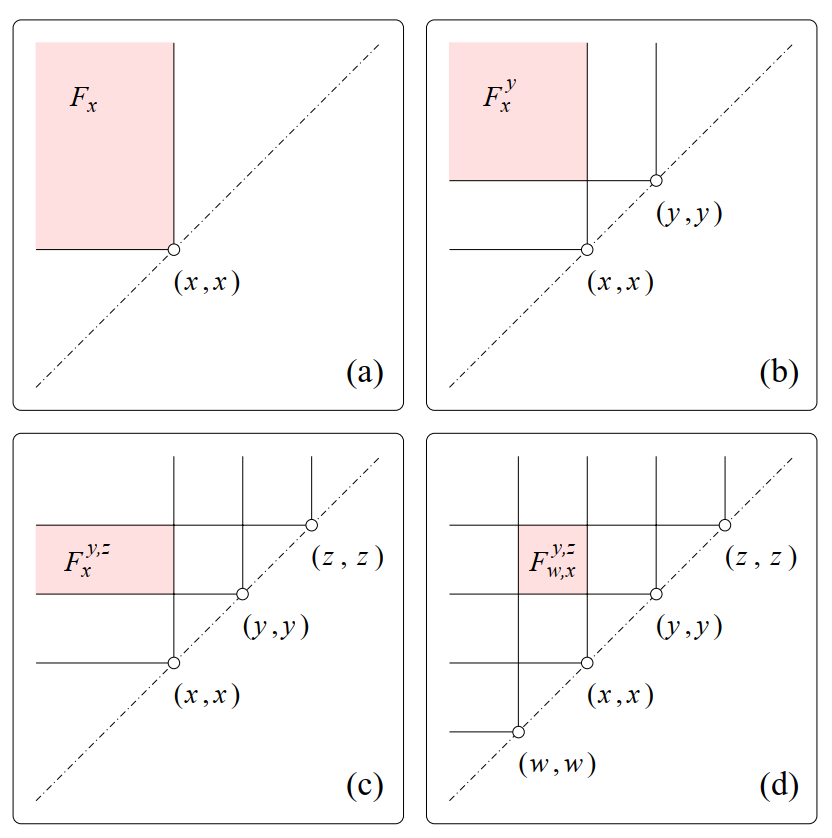
\includegraphics[width=0.6\linewidth]{figures/homology-modules.png}
    \caption[Persistent homology notation]{(From \cite{Edelsbrunner}[Figure 3]) (a) Homology modules of the sub-level set $f^{-1}(-\infty, x) $. (b) Image of $ F_x $ in $ F_y $. (c) Kernel of the surjection $ F_x^y \to F_x^z $. (d) Quotient of $ F_x^{y, z} $ and $ F_w^{y, z} $.}
    \label{fig:homology-modules}
\end{figure}

Let $ a < b < c < d \in \R $. Denote the {\bf rectangles} $ R \coloneq [a, b] \times [c, d] $, $ R_\e \coloneq [a+\e, b-\e] \times [c+\e, d -\e] $.

\begin{lemma}[Box Lemma, \cite{Edelsbrunner}] \label{lemma:box-lemma}
    With the notation above, the following inequality holds,
    \begin{align}
        \#(D(f), \cap R_\e) \leq \#(D(g) \cap R).
    \end{align}
\end{lemma}
\begin{proof}
Note that we can asume that $ a + \e < b - \e $ and $ c+\e < d - \e $. Otherwise the rectangle $ R_\e $ would not exist. Also note that
\begin{align}
    \#(D(f) \cap R_\e) &= \dim F_{a+\e, b-\e}^{c+\e, d-\e} \\
    \#(D(g) \cap R) &= \dim G_{a, b}^{c, d} \\
\end{align}
To make our proof we draw diagram \ref{cd:box}. Lets analice every element of the diagram.
\begin{equation} \label{cd:box}
\begin{tikzcd}
    G_a^d \arrow[rrr, "r_1"]
    & & & G_b^d \\
    & F_{a+\e}^{d-\e} \arrow[r, "r_2"]
    & F_{b-\e}^{d-\e} \arrow[ru, "s_1"] & \\
    & F_{a+\e}^{c+\e} \arrow[u, "u_2"] \arrow[r, "r_3"]
    & F_{b-\e}^{c+\e} \arrow[u, "u_3"'] & \\
    G_a^c \supseteq E_a^c \arrow[ru, "s_2"] \arrow[uuu, "u_1"] \arrow[rrr, "r_4"]
    & & & E_b^c \subseteq G_b^c \arrow[lu, "s_3"'] \arrow[uuu, "u_4"']
\end{tikzcd}
\end{equation}
First of all, the middle upside arrows, are
\begin{align}
    u_2 &= f_{a+\e}^{c+\e, d-\e}, \quad & u_3 &= f_{b-\e}^{c+\e, d-\e}.
\end{align}
Right arrows $ r_1, r_2, r_3, r_4 $ represent the inclusions from its respective vector spaces to their destination. The objetive is to define the respective quotients to define $ G_{a, b}^{c, d} $. Recall the inclusion maps defined in the proof of Lemma \ref{lemma:quadrant-lemma}, $ \varphi_x \colon F_x \to G_{x+\e} $ and $ \psi_x \colon G_x \to F_{x+\e}$. We define
\begin{align}
    E_b^c &\coloneq \psi_c^{-1}(F_{b-\e}^{c+\e, d-\e}) \cap G_b^c, \quad & E_a^c \coloneq G_a^c \cap E_b^c.
\end{align}
We have then that the outer upside arrows are the respective restrictions
\begin{align}
    u_1 &= g_a^{c,d}\rvert_{E_a^c}, \quad & u_4 &= g_b^{c,d}\rvert_{E_b^d}.
\end{align}
We denote
\begin{align}
    s_1 &\coloneq \varphi_{d-\varepsilon}\rvert_{F_{b-\varepsilon}^{d-\varepsilon}}, \quad & s_2 &\coloneq \psi_c\rvert_{E_a^c}, \quad & s_3 \coloneq \psi_c(G_b^c)\rvert_{E_b^c}.
\end{align}
By the inclusions \eqref{eq:quadrant-3}, we have that
\begin{align}
    \varphi_{d-\varepsilon}(F_{b-\varepsilon}^{d-\varepsilon}) &\subseteq G_b^d, \quad & \psi_c(G_a^c), &\subseteq F_{a+\varepsilon}^{c+\varepsilon} \quad & F_{b-\varepsilon}^{c+\varepsilon} &\subseteq \psi_c(G_b^c).
\end{align}
Note that by the manner we have define the diagram, it need to be that
\begin{align}
    \im(s_3) &= \ker(u_3), \quad & \im(s_1) &\subseteq G_b^d.
\end{align}
Also, we can observe that $ u_4 = s_1 \circ u_3 \circ s_3 $. As $ u_3 \circ s_3 = 0 $, then $ E_b^c = \ker(u_4) $. Also, as $ r_1 \circ u_1 = u_4 \circ r_4 = 0 $ and $ r_1 $ is the inclusion, then $ E_a^c = \ker(u_1) $. Hence, we can write
\begin{align}
    E_b^c &= E_b^{c,d} \subseteq G_b^{c,d}, \quad & E_a^c = E_a^{c,d} \subseteq G_a^{c,d}.
\end{align}  
As $ E_a^{c,d} = E_b^{c,d} \cap G_a^{c,d} $, the following quotient inclusion holds
\begin{align}
    E_{a,b}^{c,d} = E_b^{c,d} / E_a^{c,d} \subseteq G_b^{c,d} / G_a^{c,d} = G_{a,b}^{c,d}.
\end{align}
Therefore, we have
\begin{align}
    \dim(E_{a,b}^{c,d}) \leq \dim(G_{a,b}^{c,d}).
\end{align}
Now note that
\begin{align}
    E_{a,b}^{c,d} &= \ker(u_4) / \ker(u_1), \quad & F_{a+\varepsilon, b+\varepsilon}^{c+\varepsilon, d+\varepsilon} &= \ker(u_3 / \ker(u_2)).
\end{align}
By construction $s_3(\ker(u_4)) = \ker(u_3) $. As for every $x \in \ker(u_1)$, $r_2 \circ u_2 \circ s_2 (x) = u_3 \circ s_3 \circ r_4 (x) = 0 $, and $r_2 $ is an injection, then $ s_3(\ker(u_1)) = s_2(\ker(u_1) \subseteq \ker(u_2))$, we get 
\begin{align}
    \dim(F_{a+\varepsilon, b+\varepsilon}^{c+\varepsilon, d+\varepsilon}) \leq \dim(E_{a,b}^{c,d}).
\end{align}
Hence, the desired inequality is hold as we have seen that
\begin{align}
    \#(D(f) \cap R_\e) = \dim F_{a+\e, b-\e}^{c+\e, d-\e} \leq \dim(E_{a,b}^{c,d}) \leq \dim(G_{a,b}^{c,d}) = \#(D(g) \cap R).
\end{align}
\end{proof}

\begin{theorem}[Hausdorff Stability, \cite{Edelsbrunner}] \label{theorem:hausdorff-stability}
    Let $ X $ be a triangulable space, and $ f, g\colon X \to \R $ continuous tame functions. Then,
    \begin{equation}
        \dhf(D(f), D(g)) \leq \| f - g \|_\infty.
    \end{equation}
\end{theorem}
\begin{proof}
    As a direct consequence of Lemma \ref{lemma:box-lemma} if $ (x, y)\in D(f) $ then there must exist some point in $ D(g) $ at distance less than or equal to $ \varepsilon =  \| f - g \|_\infty $ from $(x, y) $ since the total multiplicity of $ D(g) \cap R_\varepsilon $ is at least one.
\end{proof}

\section{Bottleneck Stability} \label{sec:bot-stability}
In this section we are going to prove Theorem \ref{theorem:edelsbrunner-stability}. 

\Main*

\begin{definition}[Very close tame functions]
    Let $ f, g \colon X \to \R $ be tame functions. We define
    $$
        \delta_f = \min \{ \|p - q\|_\infty : p \in D(f) \setminus \Delta, \ q \in D(f), \ p \neq q\}.
    $$
    We say that $ g $ is {\bf very close} to $ f $ if $\|f-g\|_\infty < \delta_f / 2$.
\end{definition}

\begin{lemma}[Easy Bijection Lemma, \cite{Edelsbrunner}] \label{lemma:easy-biyection}
    Let $ f, g \colon X \to \R $ be tame functions, where $ g $ is very close to $ f $. Then, following holds,
    \begin{align}
        \db(D(f), D(g)) \leq \|f - g \|_\infty.
    \end{align}
\end{lemma}

\begin{proof}
    Let $ p \coloneq (a_i, a_j) \in D(f) - \Delta $ be a point in the diagram of $ f $ that is not in the diagonal, and let $ \mu \coloneq \beta_i^j $ denote its multiplicity. Let $S_\e$ be the square of center $ p $ and radius $\e = \| f- g \|_\infty $. That is, the square of side $ 2 \e $. By definition of the square $ S_\e $ we have that the number of points of its intersection with the diagram of $ g $ must be grater or equal than the multiplicity at $ p $. Hence, by the Box Lemma \ref{lemma:box-lemma} we have
    \begin{equation}
        \mu \leq \# (D(g) \cap S_\e) \leq \#(D(f) \cap S_2\e).
    \end{equation}
    As $ g $ is very close to $ f $, we have $ 2\e \leq \delta_f $. Hence $ p $ is the only point of $ D(f) $ in $ S_\e$, and therefore the previous inequality is in fact an equivalence. If there was a point in the intersection which was not in $\mu $ then it would be inside the square $ S_\e $ and meaning the distance $\| f - g \| $ would be smaller. That is
    \begin{equation}
        \mu = \# (D(g) \cap S_\e).
    \end{equation}
    Hence we can map every point in $ D(g) \cap S_\e $ with $ p $. We can then repeat this process for every other $ p \in D(f) \setminus \Delta $. After this process, every point of $ D(g) $ which have not been matched yet, must be at distance greater than $ \e $ from $ D(f) \setminus \Delta $. By Theorem \ref{theorem:hausdorff-stability}, every unmatched point must be at distance at most $ \e $ from the diagonal $ \Delta $. Hence, if we map each of this points to $ \Delta $, we have built a bijection between $ D(f) $ and $ D(g) $ that moves each point at most $ \e $.
\end{proof}

\begin{definition}
    Let $\hat f, \hat g $ be two piecewise linear functions over a simplicial complex $ K $. Let $ \lambda \in [0, 1] $. A {\bf convex combination} of $ \hat f $ and $ \hat g $ is a function of the form
    \begin{equation}
        h_\lambda \coloneq (1-\lambda) \hat f + \lambda \hat g.
    \end{equation}
\end{definition}

\begin{lemma}[Interpolation Lemma, \cite{Edelsbrunner}] \label{lemma:interpolation}
    Let $ K $ be a simplicial complex. Take two piecewise linear functions $ \hat f, \hat g \colon K \to \R $. Then, the following holds,
    \begin{align}
        \db(D(\hat f), D(\hat g)) \leq \|\hat f - \hat g \|_\infty.
    \end{align}
\end{lemma}
\begin{proof}
    Let $ c \coloneq \| \hat f - \hat g \|_\infty $. For every $ \lambda \in [0, 1] $, define $ \delta(\lambda) \coloneq \delta_{h_\lambda} > 0 $. Let $ J_\lambda $ denote open intervals around each $ \delta $ as follows, and consider the set $ C $ of all $ J_\lambda $ be
    $$
        C \coloneq \left\{J_\lambda \coloneq\left( \lambda - \frac{\delta(\lambda)}{4c}, \lambda + \frac{\delta(\lambda)}{4c}\right)\right\}.
    $$
    The set $ C $ is an open cover of the interval $ [0, 1] $. Let $ C'$ be the minimal subcover of $ C $. As $ [0, 1] $ is compact, the subcover $ C' $ must be finite. Consider then $ \lambda_1 < \lambda_2 < \cdots < \lambda_n $ the midpoints of the intervals in $ C' $. As $ C' $ is minimal, then each intersection $ J_{\lambda_i} \cap J_{\lambda_{i+1}} $ is not empty. Hence
    $$
        \lambda_i + \lambda_{i+1} \leq \frac{\delta(\lambda_i) + \delta(\lambda_{i+1})}{4c} \leq \frac{\max\{\delta(\lambda_i), \delta(\lambda_{i+1})\}}{2c}.
    $$
    Therefore, by definition of $ c $ and each $ h_{\delta_i} $, it holds
    $$
        \|h_{\delta_i} - h_{\delta_{i+1}} \|_\infty = c(\lambda_{i+1} - \lambda_i) \leq \frac{\max\{\delta(\lambda_i), \delta(\lambda_{i+1})\}}{2}.
    $$
    This implies that $ h_{\delta_i} $ is very close to $ h_{\delta_{i+1}} $ or viceversa. Then, by Lemma \ref{lemma:easy-biyection}, for every $ 1 \leq i \leq n-1 $,
    \begin{align} \label{eq:picewise-inequality}
        \db(D(h_{\lambda_i}), D(h_{\lambda_{i+1}})) \leq \| h_{\lambda_i} - h_{\lambda_{i+1}} \|_\infty.
    \end{align}
    Let $ \lambda_0 = 0 $ and $ \lambda_{n+1} = 1 $. Then $ h_{\lambda_0} = \hat f $ is very close to $ h_{\lambda_1} $ and $ h_{\lambda_1} = \hat g $ is very close to $ h_{\lambda_n} $ and therefore \eqref{eq:picewise-inequality} also holds for $ i = 0 $ and $ i = n+1 $. Finally, using the triangle inequality we have
    $$
        \db(D(\hat f), D(\hat g)) \leq \sum_{i=0}^{n} \db(D(h_{\lambda_i}), D(h_{\lambda_{i+1}})) \leq \sum_{i=0}^{n} \| h_{\lambda_i} - h_{\lambda_{i+1}} \|_\infty = \|\hat f - \hat g \|_\infty.
    $$
\end{proof}

For the final proof lets recall what the star of a simplicial complex is.

\begin{definition}[Star of a simplicial complex]
    Let $\sigma $ be a simplex in a simplicial complex $ L $. The {\bf star} $ \st(\sigma) $ of $ \sigma $ is the set of simplices in $ L $ which contain $ \sigma $ as a face. The {\bf star of a subset} $ K $ of $ L $, denoted $ \st(K) $, is the union of the stars of each simplex of $ K $.
\end{definition}

\Main*
\begin{proof}
    As $ X $ is triangulable, there exists a finite simplicial complex $ L $ and a homeomorphism $ \Phi\colon L \to X $. Hence a persistence diagram is invariant under this change of variables. That is, $ f \circ \Phi\colon L \to \R $ is tame and $ D(f \circ \Phi) = D(f) $. Since $ f $ and $ g $ are continuous and $ L $ is compact, for every $ \delta < 0 $ there exists a subdivision $ K $ of $ L $ such that for every $ u, v $ points of a common simplex $ \sigma \in K $, 
    \begin{align}
        |f \circ \Phi (u) - f \circ \Phi(v)| &\leq \delta, \\
        |g \circ \Phi (u) - g \circ \Phi(v)| &\leq \delta.
    \end{align}
    Let $ \hat f, \hat g \colon \st(K) \to \R $ be the piecewise linear interpolations of $ f \circ \Phi $ and $ g \circ \Phi $ on $ K $. By construction of $ K $ and the definition of the $ L_\infty$-norm, these interpolations satisfy
    \begin{align}
        \| \hat f - f \circ \Phi \|_\infty &\leq \delta, \\
        \| \hat g - g \circ \Phi \|_\infty &\leq \delta.
    \end{align}
    Hence, by Lemma \ref{lemma:interpolation} and the triangle inequality
    \begin{equation}
        \db(D(\hat f), D(\hat g)) \leq \|\hat f - \hat g \|_\infty \leq \| f \circ \Phi - g \circ \Phi \|_\infty + 2 \delta \leq \| f - g \|_\infty + 2 \delta.
    \end{equation}
    Now, we can take some $ \delta $ such that $ \delta \leq \delta_f/2 $ so $ \hat f $ is very close to $ f $. This allows us to use Lemma \ref{lemma:easy-biyection} to make a bijection that satisfies
    \begin{equation}
        \db(D(f), D(\hat f)) \leq \db(D(f \circ \Phi), D(\hat f)) \leq \delta.
    \end{equation}
    Analogously, also assuring $ \delta < \delta_g $ we also have
    \begin{equation}
        \db(D(g), D(\hat g)) \leq \db(D(g \circ \Phi), D(\hat g)) \leq \delta,
    \end{equation}
    and therefore, by triangle inequality again,
    \begin{equation}
        \db(D(f), D(g)) \leq \db(D(f), D(\hat f)) + \db(D(\hat f), D(\hat g)) + \db(D(\hat g), D(g)) \leq 4 \delta.
    \end{equation}
    As this holds for any $ \delta $ smaller that $ \delta_f $ and $ \delta_g $, taking the limit when $ \delta $ tends to $ 0 $, we complete the proof.
\end{proof}